\documentclass[12pt]{article}
\usepackage[utf8]{inputenc}
\usepackage{longtable}
\usepackage{multirow}
\usepackage{graphicx}
\graphicspath{ {./author/} }

\renewcommand{\baselinestretch}{1.5}

\title{John Hopcroft(1939-?)}
\author{Luis Diego Jiménez Delgado}
\date{Agosto 12 del 2019}

\begin{document}

\maketitle

\begin{center}
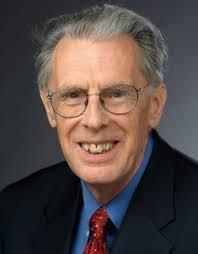
\includegraphics{ho}
\end{center}
Recibió su licenciatura por la Universidad de Seattle en 1961, y sus títulos de máster y doctorado por la Universidad de Stanford en 1962 y 1964, respectivamente. A partir de entonces trabajó durante tres años en la Universidad de Princeton. Desde entonces ha permanecido en la Universidad de Cornell, donde en 2006 es el Profesor IBM de Ingeniería y Matemática Aplicada en Ciencias de la Computación.
Recibió el Premio Turing de la ACM--el galardón más prestigioso que se concede en su campo--junto con Robert Tarjan en 1986, "por logros fundamentales en el diseño y análisis de algoritmos y estructuras de datos." Además de su labor investigadora, es bien conocido por sus libros sobre algoritmos y lenguajes formales, escritos junto con Jeffrey Ullman y Alfred Aho, siendo sus títulos considerados como textos clásicos en el campo.
\end{document}